\documentclass[conference]{IEEEtran}
\usepackage{cite}
\usepackage{amsmath,amssymb}
\usepackage{graphicx}
\usepackage{booktabs}
\usepackage{url}
\usepackage{microtype}

\graphicspath{{../draft/figures/}}

\begin{document}

\title{Testing Input Evidence and System One Decisions in Misinformation Classification: Pre-registered Fine-Tuning of a Typed-Decision Vision-Language Model across Three Benchmarks}

\author{\IEEEauthorblockN{Ananya Saravani Ganni, Harika Etikela, Rafiul Haider, and Krishna Bathula}
\IEEEauthorblockA{Pace University\\
Analytics Capstone, Fall 2026}}

\maketitle

\begin{abstract}
Multimodal misinformation is false in structurally different ways, yet benchmarking is fragmented across incompatible evaluation protocols and cost disclosure is rare. We report a pre-registered study of LAYA-Vision, a 201M-parameter typed-decision vision-language model, in two registered parts. In Part I, fine-tuning on 490 examples reaches 0.6020 macro-F1 on the official MMFakeBench test split, scored exactly once: above every directly compared fine-tuned system on that protocol and below only a frontier-model agent system, at about \$0.04 per 1,000 predictions. The gain is dataset-conditional. The same recipe is null on NewsCLIPpings (0.5104 accuracy against a 0.5141 baseline) and near-flat in transfer to VERITE (0.3506 against 0.3467). In Part II, a registered probe tests whether retrieved evidence rescues the factual benchmarks, at inference time and in training. It does not, under abstention accounting: the one headline gain is an abstention collapse, in which the evidence-trained model labels 294 of 300 probe items pristine and scores falsified accuracy of exactly 0 of 148. A scale probe at 10,040 training items shows the NewsCLIPpings null is not a data-size artifact. The study contributes an abstention-accounting standard for arbitrated verdicts and a set of measured warnings for benchmark users, including a 0.9150 metadata leakage ceiling on MMFakeBench and a calibration-transfer harm. All negative results are reported unsoftened, with a complete cost ledger.
\end{abstract}

\section{Introduction}

A social-media post pairs an image with a caption, and the pair can be false in structurally different ways: the text can distort facts, the image can be manipulated or miscaptioned, and two authentic items can be placed together out of context. A useful detector should say not only whether a pair is false but how it is false. Benchmarks operationalize this typology with different label spaces and native metrics: MMFakeBench \cite{Liu2024MmfakebenchMixedsource}, NewsCLIPpings \cite{Luo2021NewsclippingsAutomatic}, and VERITE \cite{Papadopoulos2023VeriteRobust}. Most visible progress comes from large vision-language models and agent frameworks that assume frontier APIs, external retrieval, or test-time search, report under incompatible split and metric regimes, and rarely disclose cost \cite{Radford2021LearningTransferable,Qi2024SnifferMultimodal}. Fine-tuned detectors are a smaller alternative, and parameter-efficient recipes such as LoRA \cite{Hu2021LoraLowrank} make small-data adaptation cheap, but split conventions are often unstated and hyperparameters are seldom pre-registered, so stability and transfer are hard to audit.

This paper reports a pre-registered study of LAYA-Vision, a 201M-parameter typed-decision vision-language model. A typed-decision model reads a structured state plus a typed question and returns calibrated probabilities over a fixed option set in a single forward pass; it generates no free text. Every evaluation call answers two questions at once: a native choice question over the dataset pack's classes, and a binary fake screen. The choice verdict headlines; disagreement between the two answers is labelled uncertain, and that arbitration rule drives several of the study's findings.

The thesis is that adaptation gains are dataset-conditional. Part I fine-tunes the model under one frozen protocol across the three benchmarks and finds one strong result, one null, and one flat transfer. Part II, registered after Part I and reported in the same paper, tests the remedy the Part I diagnosis suggests: if NewsCLIPpings and VERITE falsity is per-item and factual, external evidence supplied at inference time, or taught in training, should help where fine-tuning on style cannot. It does not, and the reason it appears to at first glance is the study's main methodological finding. Two contributions are named so they can be cited as such: an \textbf{abstention-accounting standard} for arbitrated verdicts (Section~\ref{sec:abstention}), and a \textbf{warnings section} for benchmark users (Section~\ref{sec:warnings}).

\section{Related Work}

Large vision-language models and agent frameworks dominate visible progress on multimodal misinformation. Contrastive pretraining \cite{Radford2021LearningTransferable} and instruction-tuned assistants provide strong zero-shot representations, and agent wrappers compose these models with tools and retrieval: SNIFFER, for example, retrieves external knowledge for out-of-context detection \cite{Qi2024SnifferMultimodal}, and MMD-Agent integrates reasoning and tool use on MMFakeBench \cite{Liu2024MmfakebenchMixedsource}. These systems commonly assume frontier APIs, external retrieval, or test-time search, and their results are often reported under different split and metric regimes. Evidence-based claim verification is the older line behind Part II's design \cite{Thorne2018FeverLargescale}. Fine-tuned detectors and parameter-efficient adaptation \cite{Hu2021LoraLowrank} are the smaller alternative this study audits: our work is not an agent system but a single forward-pass typed-decision classifier with zero external dependencies, explicit split labels, and disclosed costs. On calibration and dataset bias, our findings are concrete instances of known failure modes: calibration degrades under distribution shift \cite{Guo2017CalibrationModern,Ovadia2019CanYou,Minderer2021RevisitingCalibration}, annotation artifacts create shortcuts \cite{Gururangan2018AnnotationArtifacts}, and leakage and reproducibility failures are widespread in machine-learning-based science \cite{Kapoor2023LeakageReproducibility,Pineau2020ImprovingReproducibility}. Dataset documentation standards such as datasheets support the disclosure this study practices \cite{Gebru2018DatasheetsDatasets}.

\section{Protocol}

Dataset packs fix the questions, label spaces, native metrics, and calibration behaviour before any scoring (Table~\ref{tab:packs}). Every evaluation call answers two typed questions in one forward pass: the pack's native choice question, whose verdict headlines, and a binary fake screen expressed as a probability question. Where the two answers disagree on the fake side, the arbitrated verdict is uncertain; that single rule is what makes abstention a measurable quantity throughout the study, rather than a post hoc label. MMFakeBench uses four classes (original, textual veracity distortion, visual veracity distortion, mismatch) and macro-F1; NewsCLIPpings uses pristine against falsified and accuracy; VERITE uses truthful, miscaptioned, and out-of-context and three-class accuracy. Metrics are never averaged across datasets. Gold labels, item IDs, file paths, and source metadata are never model inputs.

\begin{table}[t]
\centering
\caption{Dataset packs: label spaces, native metrics, evaluation sets.}
\label{tab:packs}
\begin{tabular}{llll}
\toprule
Pack & Classes & Metric & Evaluation set \\
\midrule
MMFakeBench & 4 & macro-F1 & official test, 9,999 rows \\
NewsCLIPpings & 2 & accuracy & streamed validation, 7,024 rows \\
VERITE & 3 & accuracy & local extraction, 1,001 rows \\
\bottomrule
\end{tabular}
\end{table}

The frozen protocol is: selection on a tune split only; the MMFakeBench test split scored exactly once, by the frozen winner, after selection; calibration fitted only on a reserved calibration split; and every training run receipted. The main grid compares a full encoder-plus-head arm (the vision tower is frozen in both arms, a library limitation recorded as an amendment) against a LoRA arm \cite{Hu2021LoraLowrank}, under the training library's two objectives (soft\_ce and rlcd, claimed only as implemented in that library) and three step budgets. A supplementary ablation tier runs after selection and never feeds it. Five hypotheses were pre-registered: H1, an MMFakeBench test gain of at least $+0.03$ macro-F1 with no per-class recall drop above 5 points; H2, a NewsCLIPpings trained arm in the 0.55 to 0.65 accuracy band; H3, VERITE transfer accuracy in the 0.38 to 0.48 band; H4, a minimum per-class tune recall of at least 0.25 for the winner; H5, calibration fitted on the reserved split bringing tune expected calibration error under 0.15 with accuracy unchanged. Part II registrations (the EvidenceGate design, the probe and carve constructions, the wording drill-down, the confirmation screen, the Wikipedia arm, the full-set VERITE scoring, the scale probe, and the tune read) were likewise written before the runs they governed.

Training uses seed 20261122, maximum sequence length 1024, batch size 8, and bf16 precision. The MMFakeBench development partition is carved from the official 1,000-item validation split as 490 train items, 105 tune items, and 105 calibration items, each item in both question forms. The NewsCLIPpings arm is carved from the official train split only (2,001 train items); its evaluation streams the official validation rows. Table~\ref{tab:hypotheses} states the five verdicts up front; the sections that follow give the evidence.

\begin{table}[t]
\centering
\caption{Pre-registered hypotheses and verdicts.}
\label{tab:hypotheses}
\begin{tabular}{lll}
\toprule
Hypothesis & Claim in brief & Verdict \\
\midrule
H1 & MMFakeBench gain $\geq +0.03$ & MET \\
H2 & NewsCLIPpings arm in band & NOT MET \\
H3 & VERITE transfer in band & NOT MET \\
H4 & Recall floor $\geq 0.25$ & MET \\
H5 & Calibration, as registered & MET, qualified \\
\bottomrule
\end{tabular}
\end{table}

\section{Part I: Fine-Tuning across Three Benchmarks}

\subsection{MMFakeBench: the win}

The frozen winner is the full encoder-plus-head arm with soft\_ce at 735 steps, tune macro-F1 0.7389. Within this library's two objectives and under this recipe, soft\_ce beats rlcd in all six matched pairs. On the official test split, scored exactly once on 9,999 paired rows, the winner reaches macro-F1 0.6020 against a pretrained baseline of 0.2037: a paired-resampling difference of $+0.3983$ with 95\% interval $[+0.3853, +0.4108]$, and every per-class recall improves (test recalls: original 0.617, textual distortion 0.834, visual distortion 0.512, mismatch 0.422). H1 and H4 are met (the winner's minimum per-class tune recall is 0.6129). The winner's remaining errors concentrate on the original-versus-mismatch boundary (2,375 of 3,870 errors), and its validation-to-test accuracy gap (0.7690 against 0.6130) is consistent with selection on a 105-item tune split rather than a protocol failure, because the baseline is nearly flat across the same two splits.

The supplementary tier, which runs after selection and never feeds it, bounds the result's fragility. A second seed of the winner recipe reaches tune macro-F1 0.7320, so the winner is not a lucky-seed artifact at the tune level. The data-size curve at a fixed 490 steps collapses at 122 training items (0.1168), recovers at 245 items (0.3670), and reaches 0.6598 at 490 items: a minimum-data cliff under this recipe. LoRA rank is a stability hazard at this scale: rank 8 and rank 16 stay trainable, while rank 32 collapses (0.1168 at 490 steps, 0.2244 at 735 steps, with training loss rising). Head-only fine-tuning scores at most 0.4899 and is never competitive.

\begin{table}[t]
\centering
\caption{MMFakeBench grid selection on the tune split (105 items).}
\label{tab:grid}
\begin{tabular}{lcc}
\toprule
Configuration & Tune F1 & Tune acc \\
\midrule
full\_soft\_ce\_735 & 0.7389 & 0.7429 \\
lora\_soft\_ce\_735 & 0.7187 & 0.7048 \\
full\_soft\_ce\_490 & 0.6598 & 0.6667 \\
lora\_soft\_ce\_245 & 0.6282 & 0.6571 \\
full\_rlcd\_735 & 0.6061 & 0.6190 \\
full\_soft\_ce\_245 & 0.5954 & 0.6000 \\
full\_rlcd\_490 & 0.5880 & 0.6000 \\
lora\_soft\_ce\_490 & 0.5726 & 0.5810 \\
full\_rlcd\_245 & 0.5667 & 0.5619 \\
lora\_rlcd\_245 & 0.4597 & 0.5905 \\
lora\_rlcd\_490 & 0.4505 & 0.6095 \\
lora\_rlcd\_735 & 0.1946 & 0.3333 \\
\bottomrule
\end{tabular}
\end{table}

\begin{table}[t]
\centering
\caption{Protocol A (official MMFakeBench test) comparison, macro-F1 in percent as published. Only the frontier agent system sits above this study's 201M model; every fine-tuned system on the verified official test split sits below it.}
\label{tab:protocol}
\begin{tabular}{lc}
\toprule
System & Macro-F1 (\%) \\
\midrule
GPT-4V + MMD-Agent & 61.5 \\
\textbf{LAYA-Vision (this study)} & \textbf{60.20} \\
SCPO & 57.3 \\
GPT-4V Standard & 48.8 \\
LLaVA-1.6-34B Standard & 25.7 \\
\bottomrule
\end{tabular}
\end{table}

Table~\ref{tab:protocol} places the result among published systems on the same protocol. The comparison needs the protocol label before it needs error bars: the wider literature is fragmented across at least six incompatible regimes (validation, binary, retrieval, and private re-split numbers are not comparable), and we table only verified official-test results here. Inference is measured at 0.16 seconds per item, about \$0.04 per 1,000 predictions, with zero external dependencies.

\subsection{NewsCLIPpings and VERITE: the null and the flat transfer}

The same recipe does not transfer to per-item factual pairing. On NewsCLIPpings, the trained arm scores accuracy 0.5104 on the 7,024 streamed validation rows against the baseline's 0.5141: a null result (H2 not met). Macro-F1, not the pack's native metric, moves the other way (0.4036 to 0.4436) on a rebalancing toward pristine; the registered verdict reads on accuracy, and on accuracy nothing moves. The trained model's screen AUC is 0.529 and its mean confidence sits near 0.500, so it learns no useful confidence-separated boundary. On VERITE, the MMFakeBench winner transferred without any VERITE training reaches accuracy 0.3506 against the baseline's 0.3467 (H3 not met): it differs from the baseline on 543 of 1,001 labels yet nets $+0.4$ points, which is label churn, not transfer. Fig.~\ref{fig:headline} collects the three before-and-after headlines on their native metrics.

\begin{figure*}[t]
\centering
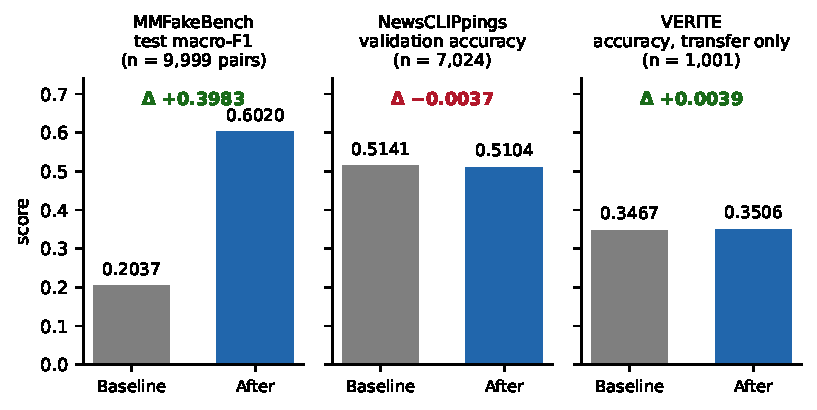
\includegraphics[width=\textwidth]{fig_headline.pdf}
\caption{Before-and-after headline results, one panel per dataset, each on its native metric. Left: MMFakeBench test macro-F1, baseline 0.2037 to winner 0.6020. Centre: NewsCLIPpings validation accuracy, baseline 0.5141 to trained 0.5104, a null result. Right: VERITE accuracy under transfer only, baseline 0.3467 to 0.3506, near-flat. The three metrics are never averaged across datasets.}
\label{fig:headline}
\end{figure*}

\subsection{Calibration, and a leakage ceiling}

Calibration is a property of the model and distribution pair, not of the model alone \cite{Guo2017CalibrationModern,Ovadia2019CanYou,Minderer2021RevisitingCalibration}. On the reserved calibration split, fitted scaling reduces expected calibration error from 0.2664 to 0.0865 with accuracy unchanged, so H5 is met as registered. The qualification is part of the claim: the same fitted temperature ($T=8.4214$) applied to held-out validation worsens ECE from 0.1056 to 0.3955, while a distribution-matched split-half fit ($T\approx1.65$) improves it from 0.0994 to 0.021. Both published packs therefore ship at $T=1.0$.

Separately, a rule that reads only the two provenance fields \texttt{text\_source} and \texttt{image\_source} reaches 0.9150 macro-F1 on the MMFakeBench tune split. That metadata leakage ceiling is reported as a benchmark warning, not a model result; the model itself never receives source metadata. Leakage and reproducibility failures of this kind are widespread \cite{Gururangan2018AnnotationArtifacts,Kapoor2023LeakageReproducibility,Pineau2020ImprovingReproducibility}, and dataset documentation standards exist to expose them \cite{Gebru2018DatasheetsDatasets}.

\section{Part II: Evidence at Inference and in Training}
\label{sec:part2}

\subsection{EvidenceGate and its instrument failure}

EvidenceGate wraps the Part I model in a state machine: an item is routed, by pack and by an uncertainty trigger, to a pair-only judgement or to retrieval followed by a judgement with the evidence block in context, then through the same choice-and-screen arbitration. Detached, the gate is byte-identical to the Part I pipeline; that was verified, not assumed. The probe set is 300 NewsCLIPpings validation items (152 pristine, 148 falsified), stratified under seed 20261122. Arms are P0 (pair-only), P1A (evidence pool with fact-check domains excluded), P2A (the same pool, fact-check domains included), and P1B (a second retrieval variant, fact-check excluded).

The instrument failed before it measured anything. The first retrieval pass ran about 23 concurrent query streams, tripped the search backend's suspension, and returned empty result lists in silence for most items (481 of 600 probe pools empty). The repair ran serially with a circuit breaker and per-pair disk checkpointing, after a first repair attempt lost 400 repaired pairs held only in memory. After assembly and exclusions, headline evidence coverage was 193 of 300 probe items (64.3\%). A reproducibility audit then re-retrieved the pilot items fresh one day later and found mean Jaccard overlap of 0.2161 against the frozen pools: live retrieval is not reproducible at a one-day lag, so every Part II number is computed against frozen, hashed snapshots.

A 30-item pilot ran first, with no verdict registered at that size: pair-only headline accuracy 0.3667, evidence 0.4000 (paired difference $+0.0333$, interval $[-0.0667, +0.1667]$). The pair-only labels agreed with the frozen Part I comparator on 29 of 30 items, which verified that the pipeline reproduced the Part I winner's behaviour before any larger run depended on it. The gate's uncertainty trigger fired on every pilot item, a finding about the trigger threshold against this model's confidence distribution rather than about the gate's plumbing: at its registered threshold the trigger is not a selective routing device.

\subsection{Stage A: evidence at the frozen model}

The Part I NewsCLIPpings winner judged the probe items pair-only and with evidence. The paired difference for P1A against P0 is $+0.0200$ with interval $[-0.0267, +0.0667]$ under headline accounting, and the including-uncertain gap is of the same size (0.5300 against 0.5133). The verdict is NOT POSITIVE: the estimate is small, its interval crosses zero under both accountings, and the strata cut the other way, with falsified accuracy falling as evidence strengthens (0.9259 with no evidence, 0.8205 with binding evidence, 0.6727 with corroboration only). That gradient is descriptive, not causal, because stratum membership is a property of the item. At fixed coverage the evidence arm is modestly ahead at every level (0.5375 against 0.4958 at 80\% coverage; among decided items 0.5533 against 0.5039), which is why Stage A reads as a small unconfirmed effect rather than a pure accounting artifact; Stage B, next, is the artifact.

\subsection{Stage B: evidence in training, and the pristine collapse}

Stage B fine-tuned the base checkpoint on a 500-item carve with each item's assembled evidence in context, the carve disjoint from the probe in items and images. Its screen temperature and threshold were fitted on a reserved 100 calibration items only and frozen before the probe was scored (temperatures 0.0328 pair-only and 0.0300 evidence, both near the fit floor because the tuned screen is near chance on calibration items; thresholds 0.5456 and 0.5200). Table~\ref{tab:stageab} gives both stages' audited probe tables. Headline accounting gives the Stage B evidence arm a gain of $+0.2467$, interval $[+0.2000, +0.2967]$. The gain does not survive its own table, and Fig.~\ref{fig:money} shows why. Accuracy including uncertain is flat (0.5133 against 0.5167). The pair-only arm abstains on 155 items and the evidence arm on 6, a decided fraction of 0.4833 against 0.9800, and among decided items pair-only is slightly ahead (0.5241 against 0.5102). At every fixed coverage level the arms sit within 0.014 of each other. The headline gap is produced entirely by how often each arm commits.

The diagnosis is sharper than the accounting. The evidence model's choice head labels 294 of 300 items pristine; of 148 gold-falsified items it labels 4 falsified, and the arbitration then nulls all 4, so falsified accuracy under headline accounting is exactly 0 of 148. The 0.5000 headline is carried entirely by pristine items. Evidence training mostly taught the model to commit, and to commit to pristine. The carve's tune slice repeats the pattern at selection size: headline $+0.29$ for the evidence arm, interval $[0.20, 0.38]$, while including-uncertain the pair-only arm is ahead (0.55 against 0.50) and the evidence arm labels all 100 tune items pristine.

\begin{table}[t]
\centering
\caption{Audited probe tables (300 items). Stage A: frozen Part I winner. Stage B: evidence-trained checkpoint. P2A is numerically identical to P1A in both stages, for the reason given in the text.}
\label{tab:stageab}
\begin{tabular}{llccc}
\toprule
Stage & Arm & Headline & Incl.\ unc. & Unc. \\
\midrule
A & P0 pair-only & 0.4300 & 0.5133 & 44 \\
A & P1A evidence & 0.4500 & 0.5300 & 56 \\
A & P1B evidence & 0.3800 & 0.5067 & 80 \\
\midrule
B & P0 pair-only & 0.2533 & 0.5167 & 155 \\
B & P1A evidence & 0.5000 & 0.5133 & 6 \\
B & P1B evidence & 0.5067 & 0.5067 & 0 \\
\bottomrule
\end{tabular}
\end{table}

\begin{figure*}[t]
\centering
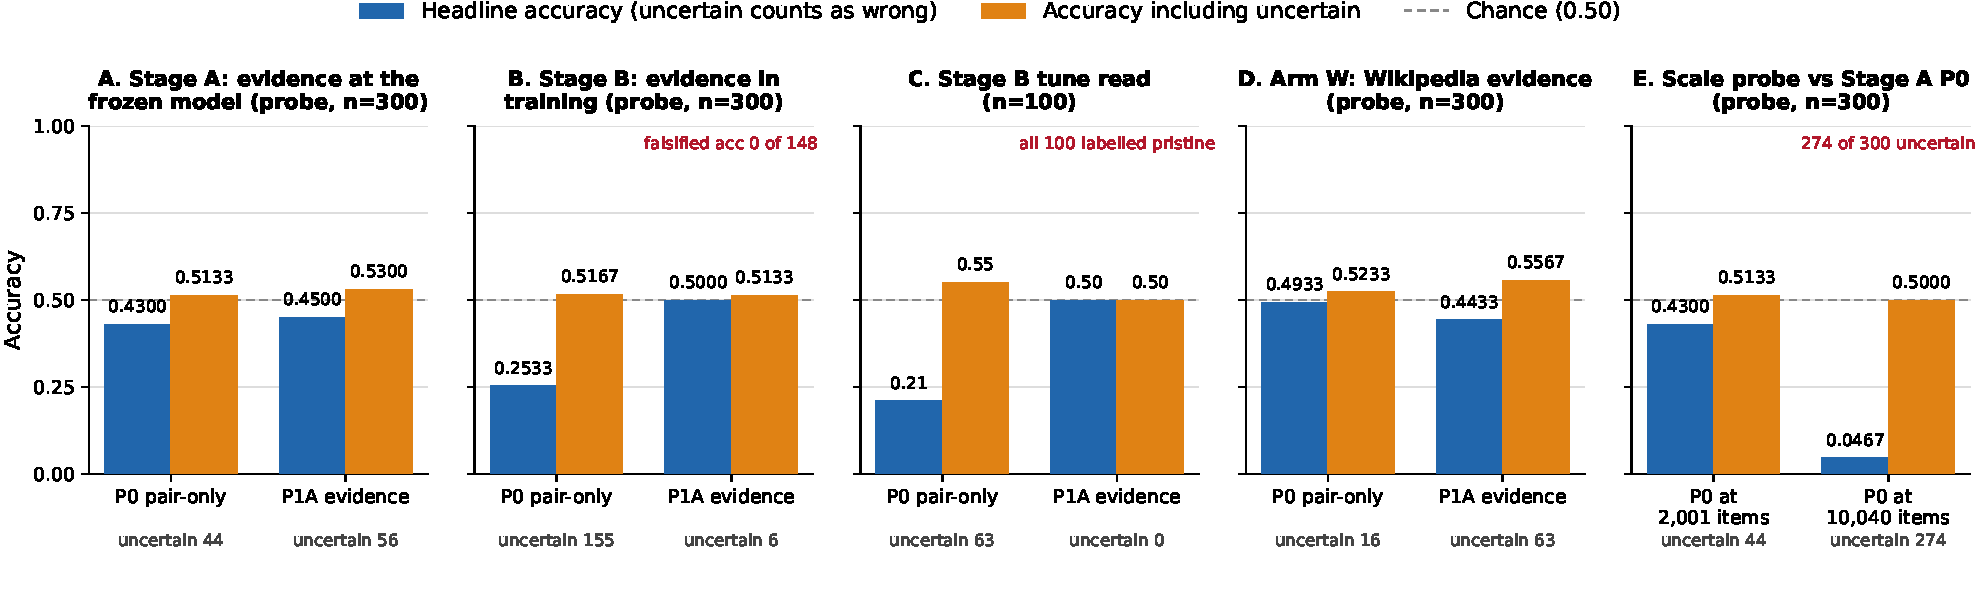
\includegraphics[width=\textwidth]{fig_money.pdf}
\caption{Headline accuracy beside accuracy including uncertain, for every headline arm comparison in Part II. The accounting rule, in plain words: headline accuracy counts every item the arbitration labels uncertain as wrong; accuracy including uncertain scores those items by the model's own screen instead, so the two bars for an arm differ only in how its abstentions are scored. Where a gap between arms appears in the blue bars and vanishes or inverts in the orange bars, the gap was a movement in how often the model committed, not in how often it was right. Panel B is the worked example: the evidence arm's headline gain of $+0.2467$ coexists with falsified accuracy of 0 of 148. Panel E shows the scale probe's collapse running the other way, into abstention: at 10,040 training items the model is uncertain on 274 of 300 items. Uncertain counts are printed under each arm.}
\label{fig:money}
\end{figure*}

\begin{table}[t]
\centering
\caption{Stage B per-class reads (300 probe items; gold 152 pristine, 148 falsified). Choice recall scores the choice head alone; headline recall scores the arbitrated verdict. The pair-only arm's correct falsified choices are all nulled by arbitration; the evidence arm's choice head almost never chooses falsified.}
\label{tab:stagebclass}
\begin{tabular}{llcc}
\toprule
Arm & Class & Choice rec. & Headline rec. \\
\midrule
P0 & pristine & 0.5000 & 0.5000 \\
P0 & falsified & 0.5338 & 0.0000 \\
P1A & pristine & 0.9868 & 0.9868 \\
P1A & falsified & 0.0270 & 0.0000 \\
P1B & pristine & 1.0000 & 1.0000 \\
P1B & falsified & 0.0000 & 0.0000 \\
\bottomrule
\end{tabular}
\end{table}

A scorer defect was found and corrected in the same stage. The Stage B scorer kept its thresholds in a module-level store that its main routine overwrote, so cross-stage deltas were computed by rescoring Stage A predictions at Stage B thresholds; the stored cross-stage figure of $+0.4367$ is exactly that artifact (Stage A evidence accuracy rescored from 0.4500 to 0.0633). An audit recomputed every Stage A and Stage B figure from the prediction files through one code path and reproduced every arm figure exactly; the corrected cross-stage difference is $+0.0500$, interval $[-0.0533, +0.1533]$. One audit item is recorded as untested rather than negative: arms P1A and P2A are numerically identical because no fact-check-domain passage survived into any of the 193 non-empty probe evidence sets, so the fact-check-inclusion contrast was never exercised.

\subsection{VERITE four arms, the Wikipedia arm, and the scale probe}

On VERITE, a group-aware split froze a held-out 200 (Table~\ref{tab:verite4}). ADAPTED minus TRANSFER is $+0.010$ with interval $[-0.080, +0.095]$, so the registered success criterion is NOT MET. Scored later on the full local set, BASE reads 0.3526 and TRANSFER 0.3586 as clean zero-shot descriptives; ADAPTED's 0.4725 is inflated by construction (801 of the 1,001 rows are its train and tune side) and its clean read stays the held-out 0.330. The adapted checkpoint used for that scoring was itself reconstructed after the original pull was found truncated, and its retraining receipt matches the original run's log to full float precision, with labels agreeing on all 200 held-out items.

\begin{table}[t]
\centering
\caption{VERITE four arms on the held-out 200. BASE here is the base checkpoint on the held-out 200 only, not the Part I full-set baseline. BASE and EVIDENCE never predict miscaptioned at all; ADAPTED is the only arm that uses all three labels at volume.}
\label{tab:verite4}
\begin{tabular}{lcc}
\toprule
Arm & Accuracy & Macro-F1 \\
\midrule
BASE & 0.285 & 0.2154 \\
TRANSFER (Part I winner) & 0.320 & 0.2855 \\
EVIDENCE & 0.325 & 0.2497 \\
ADAPTED (245 steps) & 0.330 & 0.3310 \\
\bottomrule
\end{tabular}
\end{table}

Arm W replaced live retrieval with a frozen Wikipedia corpus (an FTS5 index of 6,806,684 articles) and replicated Stage B. The paired headline difference is $-0.0500$, interval $[-0.1167, +0.0200]$; at plain 0.5 thresholds the sign flips ($+0.0267$, interval crossing zero). There is no reliable headline effect. The solid finding is the mirror image of Stage B: this model's pair-only arm shows no pristine collapse (falsified accuracy 0.9122, against 0.0 for the live-web Stage B model), and its evidence arm buys a small including-uncertain edge with far weaker falsified detection. Neither direction is an accuracy gain.

The scale probe closes the last escape route for the NewsCLIPpings null. It trains the pair-only recipe at 10,040 items for 4,900 steps and reads the result on the same 300 probe items through the audited path. Headline accuracy falls to 0.0467 against 0.4300 for the 2,001-item model (paired difference $-0.3833$, interval $[-0.4433, -0.3267]$), accuracy including uncertain sits at chance (0.5000 against 0.5133), and the model is uncertain on 274 of 300 items because its choice answer and its screen disagree. The verdict, registered in the run's own form: the null is not a data-size artifact, and it hardens at this scale. More data at this recipe bought disagreement, not decisions.

Two closing screen results belong here. A drill-down over eighteen frozen question wordings (six per dataset) found that fitted operating points, not wording, moved the numbers: sixteen of eighteen fitted temperatures sit at the 12.0 grid cap, and split-half refits swing across the full range. The screen implementation also applied a fitted-versus-raw comparison where the registered rule reads gains at $T=1$ and threshold 0.5; that deviation changed one deployment outright and is disclosed wherever it touches a claim. Under the corrected rule, the NewsCLIPpings and VERITE screens return their control wordings, and on the MMFakeBench confirmation items (300 validation items no screen, training run, or calibration had touched) every variant fails the registered gain leg: the best single, the direct-probability wording W1, reads a raw difference of $-0.1533$ with interval $[-0.2433, -0.0633]$, and the admissible set is empty. What replicates across item sets is W1's ranking (screen AUC 0.5744 against the control's 0.4308), not a registered gain, and the tune screen's battery preference does not replicate at all: its membership changes from $[1, 2, 4]$ to $[1, 3, 5]$ and it is inadmissible on the confirmation items under both readings.

The one durable screen result is narrower and comes from training, not wording selection. First, a small training test (245 steps per form, read on tune) picked a winner per dataset: on NewsCLIPpings the battery form (choice accuracy 0.50, battery screen AUC 0.5392); on VERITE the single original-context wording (choice accuracy 0.42, fitted accuracy 0.60); on MMFakeBench the single direct-probability wording W1 (choice accuracy 0.6571, macro-F1 0.6562, screen AUC 0.8215), ahead of its battery (0.6000, 0.6103, 0.7539). The Phase-2-winning MMFakeBench form was then frozen and judged once on the same 300 untouched confirmation items, validation only, the test split closed throughout: choice accuracy 0.5667, macro-F1 0.5292, predictions spread across all four classes with no degenerate collapse, and a screen read of AUC 0.8730 at its frozen temperature and threshold, where the base model's control screen sits at 0.4308 on the same items. Its per-class screen AUCs against original are 0.9531 (textual distortion), 0.9707 (visual distortion), and 0.7707 (mismatch): the screen is weakest exactly where the choice head is weakest. The fine-tune, not the wording alone, carries that discrimination; the wording chose what the fine-tune would teach. One provenance note travels with that result: recomputing the screen read from the stored prediction file gives AUC 0.8775 against the stored evaluation's 0.8730, no stored artifact establishes the mechanism of the difference, and the stored values, produced by the registered evaluation at run time and the lower of the two reads, are the canonical ones reported here. The NewsCLIPpings and VERITE Phase 3 reads, by contrast, came back null or below chance on held-out items, and neither dataset's screen wording result survives as a deployment.

The screen's flatness is visible inside Part II as well. Read directly on the 300 probe items, screen AUC barely moves between stages or arms: Stage A pair-only 0.5911 and evidence 0.5819; Stage B pair-only 0.5917 and evidence 0.5798. Evidence, in context or in training, did not make the screen a better discriminator on NewsCLIPpings; what it changed was how the choice head committed, which is the abstention story of Fig.~\ref{fig:money}.

\subsection{Situations faced, in brief}

Five incidents shaped this study's record, and each is part of the result. The retrieval suspension and its two-stage repair are described above. A replacement pod arrived with its GPU wedged at the driver level (the device tool saw the card while CUDA initialisation failed), and an earlier pod was never reachable at all; every later deployment ran a health gate, an actual CUDA tensor operation, before any setup work. The Stage B scorer defect, described above, was caught by insisting that a results file had to be consistent with itself, and proven by recomputing every figure from the prediction files. The abstention trap was caught the same way, by a review finding that the headline could not be produced by the table beneath it. And the drill-down's selection-rule deviation was caught by comparing the implementation against the registration text. The habit these produced generalises: a selection rule is part of the registration, an instrument's success return is not evidence that it measured anything, and a results file that contradicts itself is a finding, not a nuisance.

\section{Contribution 1: An Abstention-Accounting Standard}
\label{sec:abstention}

The Stage B and Arm W results are mirror images of one trap. An arbitration that scores disagreement as uncertain, read by a headline that scores uncertain as wrong, rewards any change that makes a model commit, including committing to a single class. The standard this study adopts, and proposes for any arbitrated verdict, is: whenever a headline metric counts an abstention as an error, four quantities are co-primary and no headline is quoted without them. They are the headline accuracy itself; the accuracy including uncertain; the decided fraction; and the per-class headline recalls. Under that standard, both headline-scale effects in Part II resolve into movements in the decided fraction, in opposite directions, and the scale probe's collapse is legible as the same phenomenon running into abstention instead of out of it. The standard is cheap to apply: it requires no new scoring pass, only that the abstention structure already present in an arbitrated system's output be reported beside its headline.

\section{Contribution 2: Warnings for Benchmark Users}
\label{sec:warnings}

Four warnings, each measured in this study, are collected here so they can be cited as a unit.

\begin{itemize}
\item \textbf{Metadata leakage ceiling.} A rule reading only \texttt{text\_source} and \texttt{image\_source} scores 0.9150 macro-F1 on the MMFakeBench tune split and 0.8510 macro-F1 on the official test split. Any MMFakeBench number reported without a metadata ban should be read against that ceiling. The audit is deliberately narrow: it does not test content-based source cues, so it demonstrates that a shortcut exists without quantifying every shortcut signal.
\item \textbf{Calibration transfer harm.} A temperature fitted on one distribution can severely harm calibration on another (held-out ECE 0.1056 to 0.3955 under a calibration-fitted temperature; 0.0994 to 0.021 under a distribution-matched fit). Fit on the deployment distribution, or ship $T=1.0$.
\item \textbf{Fitted operating points are fragile at small $n$.} Sixteen of eighteen fitted screen temperatures hit the grid cap, split-half refits swing across the full range, and a frozen threshold can sit one grid step wide. A screen fitted on 100 items needs its confirmation run designed in from the start.
\item \textbf{Abstention can manufacture a headline.} The Stage B gain of $+0.2467$ and its Arm W mirror are the worked examples; the accounting standard of Section~\ref{sec:abstention} is the defence. A related instrument warning: live retrieval is not reproducible at a one-day lag (mean Jaccard 0.2161), so retrieval experiments should run against frozen, hashed snapshots; and the MMFakeBench literature is fragmented across at least six incompatible protocols, so cross-paper comparisons need protocol labels before they need error bars.
\end{itemize}

\section{Threats to Validity}

The selection slices are small: 105 tune items chose the Part I winner, the drill-down screens ran on 100-item tune slices, and the probe reads rest on 300 items, so intervals around the Part II differences are wide and several verdicts are ``not confirmed'' rather than refuted at size. VERITE is scored on a local extraction of 1,001 rows of the official 1,000-item dataset, and the four-arm track's held-out 200 is a carve under this study's protocol, not the published full-set protocol; the full-set scoring narrows but does not close that gap, because the adapted arm's full-set read is inflated by construction. The study is a single-model audit: one checkpoint family and one training library. Two internal unknowns are carried openly: the identity of the library's rlcd objective against published methods of the same name is unverified, so the objective comparison is claimed only for the library objective as implemented; and the LoRA rank-32 collapse mechanism is unverified. Retrieval coverage bounds every evidence claim (64.3\% of probe items carried headline evidence), the strata gradient is descriptive rather than causal, and the fact-check-inclusion contrast is untested for the reason given in Section~\ref{sec:part2}. One competitor figure in the wider protocol audit carries an unverified split; its ranking position is conditional and no claim rests on it.

\section{Cost and Reproducibility}

The programme is deliberately cheap, and its ledger is complete (Table~\ref{tab:cost}). Part I ran on one secure RTX 4090 pod at \$0.90 per hour: total pod spend about \$6.83, of which metered training across all 29 trainings is \$2.14. The probe's closing phase cost \$3.3391 against a \$5 phase hard stop, with its remaining session spend itemised in the full record.

\begin{table}[t]
\centering
\caption{Measured cost and operational characteristics (Part I).}
\label{tab:cost}
\begin{tabular}{ll}
\toprule
Item & Value \\
\midrule
Total pod spend & $\approx \$6.83$ \\
Metered training, 29 trainings & $\$2.14$ \\
Pod rate & $\$0.90$/hour \\
Inference latency & 0.16 s/item \\
Inference cost & $\approx \$0.04$ per 1,000 predictions \\
Artifact size & $\approx 805$ MB \\
\bottomrule
\end{tabular}
\end{table} Inference costs about \$0.04 per 1,000 predictions at 0.16 seconds per item, against an estimated \$155 to score the 10,000-item test once through a frontier API and roughly \$450 to \$750 through an agent framework. Every figure in this paper traces to a receipted artifact: pre-registrations and amendments written before the runs they governed, per-configuration receipts, frozen hashed snapshots for all retrieval inputs, and a scorer audit that recomputed the Part II tables from the prediction files. The study was executed as a single notebook run, and the notebook is the run record.

\section{Conclusion}

One study, two registered parts, one thesis. Small-data fine-tuning of a typed-decision model works where falsity is stylistic: 0.6020 macro-F1 on the official MMFakeBench test, first among trained systems on that protocol, from 490 training examples. It does not transfer to per-item factual pairing: NewsCLIPpings is null, VERITE transfer is flat, an in-benchmark adapted arm adds $+0.010$ with its interval across zero, and a fivefold scale-up of the NewsCLIPpings recipe hardens the null instead of relieving it. Retrieved evidence does not rescue the factual benchmarks either: at the frozen model its gain is small and unconfirmed, in training it is an abstention collapse, and in a frozen corpus both threshold views cross zero with opposite signs. The claims that died are reported with the same prominence as the claims that stand, including a headline produced by our own scorer defect and two deployments produced by a selection-rule deviation, both caught by review and corrected on the record. What survives every audit is the procedure itself: a pre-registered, receipted, low-cost evaluation that makes dataset conditionalities and benchmark shortcuts visible, an abstention-accounting standard without which arbitrated headlines mislead, and a warnings section that other benchmark users can cite. Adaptation gains, in this study, are dataset-conditional, and the recipe works where misinformation has a style and fails where it has only a fact.

\bibliographystyle{IEEEtran}
\bibliography{../draft/bibliography}

\end{document}
